\chapter{Linee di trasmissione}
\section{Introduzione}

In termini generici possiamo dire che una \textbf{linea di trasmissione} è il supporto fisico che permette di collegare due punti.\\ \\
Alcuni esempi possono essere:
\begin{itemize}
    \item \textbf{Cavo Coassiale}
    \item \textbf{Doppino Telefonico}
    \item \textbf{Fibra Ottica}
    \item \textbf{Microstriscia}
    \item \textbf{Guida d'Onda Metallica}
\end{itemize}
Tutte queste strutture condividono una \textbf{simmetria traslazionale}, nel senso che si individua una \textbf{direzione longitudinale} e
\textbf{ortogonale} a tale direzione, le sezioni trasversali tutte uguali tra di loro.\\ \\
Il segnale si propaga nella direzione longitudinale su distanze
che sono generalmente \textbf{grandi rispetto alle lunghezze d'onda} associate al
segnale, mentre la sezione trasversale ha sempre la stessa dimensione indipendentemente da dove essa venga misurata,
\textbf{spesso piccola rispetto alla lunghezza d'onda}, e possiamo chiederci se sia possibile introdurre una \textbf{differenza} 
\textbf{di} \textbf{potenziale} e una \textbf{corrente} con caratteristiche analoghe alle tensioni e correnti a bassa frequenza, consentendoci così di descrivere la propagazione con riferimento a sole quantità scalari.\\ \\

\subsection{Tensione}
Prendiamo ad esempio una struttura guidante costituita da due \textbf{conduttori} \textbf{elettrici} \textbf{paralleli} separati da un \textbf{dielettrico} \textbf{lineare} \textbf{omogeneo} e \textbf{non} \textbf{dispersivo}.\\  
Affinché l'integrale curvilineo che va da A a B lungo un qualsiasi percorso, giacente in una sezione trasversale, dipenda dai soli estremi di integrazione (campo conservativo), si deve avere che:

\begin{equation*}
    \vcenter{\hbox{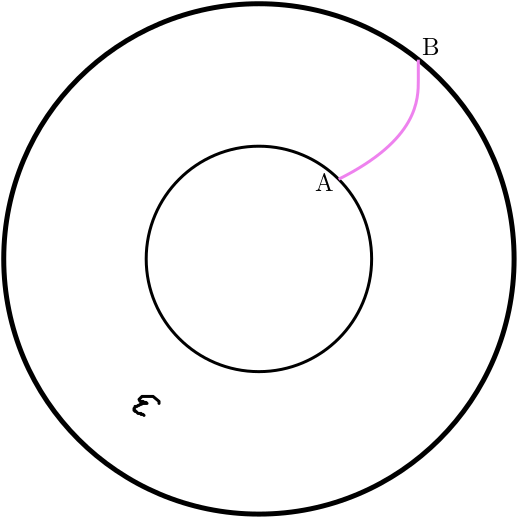
\includegraphics[width=5cm,height=5cm]{Images/figure1.png}}}
\qquad
    \int_{C(A,B)} \bar{E} \cdot \hat{\imath}_l \ dl = \varphi(A) -\varphi(B) = v(z,t)
\end{equation*}
Quindi deve accadere che per ogni curva chiusa appartenente alla sezione trasversa valga:
\begin{equation*}
\vcenter{\hbox{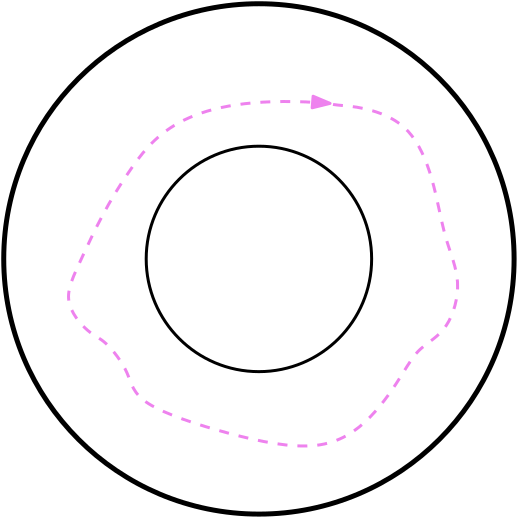
\includegraphics[width=5cm,height=5cm]{Images/figure2.png}}}
\qquad
    \color{blue}{\oint_{\partial S} \bar{E} \cdot \hat{\imath}_l \ dl = 0}
\end{equation*}
Da \textbf{Maxwell} sappiamo che:
\begin{equation*}
    \rot{\bar{E}} = -\parti{\bar{B}}{t} = -\mu \parti{\bar{H}}{t}
    \tag{Faraday-Lenz}
\end{equation*}
Che integreremo sulla superficie S\@:
\begin{equation*}
    \int_S \rot{\bar{E}} \cdot \hat{\imath}_z \ dS = \underbrace{\color{blue}{\oint_{\partial S} \bar{E} \cdot \hat{\imath}_l \ dl}}_{0} = - \frac{d}{dt} \int_s \mu \bar{H}\cdot \hat{\imath}_z \ dS 
\end{equation*}
Quindi ne consegue che $\boxed{\bar{H}\cdot \hat{\imath}_z = \bar{H}_z = 0 \; \forall \ S \ trasversa}$\\ \\

\subsection{Corrente}
Analogamente a quanto fatto prima per la tensione, per introdurre una \textbf{corrente} si deve avere:
\begin{equation*}
    \color{violet}{\oint_{\partial S} \bar{H}\cdot \bar{l} \ dl = i(z,t)}
\end{equation*}
Da \textbf{Maxwell} sappiamo che:
\begin{equation*}
    \tag{Ampere-Maxwell}
    \rot{\bar{H}} = \epsilon \parti{\bar{E}}{t} + \bar{J}
\end{equation*}
Dove $\bar{J}$ è la \textbf{corrente che circola sui conduttori}.\\
Integriamola sulla superficie S\@:
\begin{equation*}
\begin{aligned}
    &\int_S \rot{\bar{H}} \cdot \hat{\imath}_z \ dS = \color{violet}{\oint_{\partial S} \bar{H}\cdot \bar{l} \ dl} = \\
    & =\epsilon \frac{d}{dt} \int_s \bar{E}\cdot \hat{\imath}_z \ dS  + \int_s \bar{J} \ dS = \underbrace{\epsilon \frac{d}{dt} \int_s \bar{E}\cdot \hat{\imath}_z \ dS}_{\textbf{deve fare 0}}  + i(z,t)
\end{aligned}
\end{equation*}
Quindi vuol dire che:
\begin{equation*}
    \boxed{\bar{E} \cdot \hat{\imath}_z = E_z = 0 \quad \forall \ S \ trasversa}
\end{equation*}
\subsection{Campo elettrico e magnetico}
Definiamo ora il \textbf{Nabla Trasverso}:
\begin{equation*}
    \bar{\nabla}_t = \nabla - \frac{\partial}{\partial z} \cdot \hat{\imath}_z
\end{equation*}
Che ci porta queste equazioni:
\begin{equation*}
    \begin{cases}
        \bar{\nabla}_t \times \bar{E}_t = 0 & \bar{\nabla}_t \times \bar{H}_t = J_z \hat{\imath}_z\\
        \bar{\nabla}_t \cdot \bar{E}_t = \frac{\rho}{\epsilon} & \bar{\nabla}_t \cdot \bar{H}_t = 0
    \end{cases}
\end{equation*}
Quindi sostituiamo nelle Equazioni di Maxwell:
\begin{equation*}
\begin{dcases}
    \rot{\bar{E}} = \left(\bar{\nabla}_t + \frac{\partial}{\partial z} \hat{\imath}_z\right) \times \bar{E}_t = - \mu \parti{\bar{H}_t}{t}\\
    \rot{\bar{H}} = \left(\bar{\nabla}_t + \frac{\partial}{\partial z} \hat{\imath}_z\right) \times \bar{H}_t = \epsilon \parti{\bar{E}_t}{t}
\end{dcases}
\end{equation*}
\footnote{Manca J perchè circola sui conduttori verso z}
Proietto ora nel \textbf{Piano Longitudinale}:
\begin{equation*}
\tag{*}
    \begin{cases}
        \bar{\nabla}_t \times \bar{E}_t = 0\\
        \bar{\nabla}_t \times \bar{H}_t = 0
    \end{cases}
\end{equation*}
Queste equazioni stabiliscono l'\textbf{andamento dei campi rispetto alle coordinate del piano trasverso} in qualsiasi sezione danno lo stesso andamento a meno di un'\textbf{ampiezza moltiplicativa}, che ci viene data, proiettando le \textbf{Equazioni di Maxwell ridefinite} nel \textbf{Piano trasverso}:
\begin{equation*}
\tag{o}
    \begin{dcases}
    \hat{\imath}_z \times \parti{\bar{E}_t}{z} =  - \mu \parti{\bar{H}_t}{t}\\
    \hat{\imath}_z \times \parti{\bar{H}_t}{z} =  \epsilon \parti{\bar{E}_t}{t}
    \end{dcases}
\end{equation*}
\\
Quindi se valgono le (*) possiamo valutare indipendentemente il \textbf{Campo Elettrico} e il \textbf{Campo Magnetico}:\\
Integrando $\bar{E}_t$ tra A e B otteniamo:
\begin{equation*}
    v(z,t) = \int_A^B \bar{E}_t (x,y,z,t) \cdot \hat{\imath}_l \ dl
\end{equation*}
Poniamo:
\begin{equation*}
    \bar{E}_t (x,y,z) = v(z,t) \cdot \bar{e}_t (x,y)
\end{equation*}
dove:
\begin{equation*}
    \int_A^B \bar{e}_t (x,y,z,t) \cdot \hat{\imath}_l \ dl = 1
\end{equation*}
Un discorso analogo lo faremo con $\bar{H}_t$:
\begin{equation*}
    \oint_{\partial S} \bar{H}_t (x,y,z,t) \cdot \hat{\imath}_l \ dl = i(z,t)
\end{equation*}
\begin{equation*}
    \bar{H}_t (x,y,z,t) = i(z,t) \cdot \bar{h}_t (x,y)
\end{equation*}
dove:
\begin{equation*}
    \oint_{\partial S} \bar{h}_t (x,y) \cdot \hat{\imath}_l dl = 1
\end{equation*}
Sostituendo tutto nelle (o) otteniamo:
\begin{equation*}
\begin{dcases}
    \hat{\imath}_z \times \bar{e}_t \parti{v(z,t)}{z} =  - \mu \bar{h}_t \parti{i(z,t)}{t}\\
    \hat{\imath}_z \times \bar{h}_t \parti{i(z,t)}{z} =  \epsilon \bar{e}_t \parti{v(z,t)}{t}
\end{dcases}
\end{equation*}
Che riscriviamo come:
\begin{equation*}
\begin{dcases}
    \hat{\imath}_z \times \bar{e}_t \parti{v(z,t)}{z} =  - \mu \bar{h}_t \parti{i(z,t)}{t}\\
     \bar{h}_t \parti{i(z,t)}{z} = - \epsilon \hat{\imath}_z \times \bar{e}_t \parti{v(z,t)}{t}
\end{dcases}
\end{equation*}
Poniamo:
\begin{equation*}
    \hat{\imath}_z \times \bar{e}_t = - \mu \bar{h}_t \frac{\parti{i(z,t)}{t}}{\parti{v(z,t)}{z}} = A \cdot \bar{h}_t
\end{equation*}
Quindi le due equazioni diventano:
\begin{squared}
\tag{x}
\begin{dcases}
    \parti{v (z,t)}{z} = -\frac{\mu}{A} \parti{i (z,t)}{t}\\
    \parti{i (z,t)}{z} = -\epsilon\;A \parti{v (z,t)}{t}
\end{dcases}
\end{squared}
dove:
\begin{itemize}
    \item $- \frac{\mu}{A}$ è un'\textbf{induttanza}
    \item $- \epsilon A $ è una \textbf{capacità}
\end{itemize}
\section{Caso senza Perdite}
Consideriamo ora una fettina \textbf{dZ} della linea e valutiamo l'\textbf{Energia} che vi si \textbf{accumula}:\\ \\
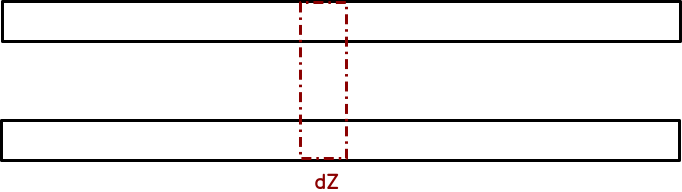
\includegraphics[width=0.4\textwidth]{Images/figure3.png}
\begin{equation*}
    \begin{aligned}
    W_e &= dz \cdot \int_S \frac{1}{2} \epsilon |\bar{E}_t|^2 dS = \frac{1}{2} dz \epsilon {(v(z,t))}^2 \int_{s_t} |\bar{e}_t|^2 dS = \\
    &= \frac{1}{2} C v^2 dz \implies C = \epsilon \int_{s_t} |\bar{e}_t|^2 dS
    \end{aligned}
\end{equation*}
\begin{equation*}
    \begin{aligned}
    W_m &= dz \cdot \int_S \frac{1}{2} \mu |\bar{H}_t|^2 dS = \frac{1}{2} dz \mu {(i(z,t))}^2 \int_{s_t} |\bar{h}_t|^2 dS = \\
    &= \frac{1}{2} L i^2 dz \implies L = \mu \int_{s_t} |\bar{h}_t|^2 dS
    \end{aligned}
\end{equation*}
Possiamo quindi costruire un \textbf{circuito} \textbf{equivalente} a questa fettina, permettendoci di individuare facilmente le equazioni che legano \textbf{tensioni} e \textbf{correnti}:
\begin{center}
    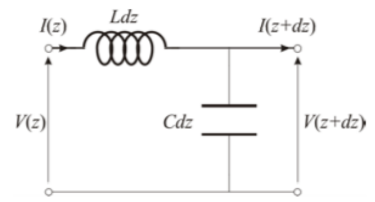
\includegraphics[width=0.4\textwidth]{Images/figure4.png}
\end{center}
Analizziamo la \textbf{maglia}:
\begin{equation*}
    \begin{cases}
    V(z) = j\w L dz I(z) + V(z+dz)\\
    V(z+dz) - V(z) = - j\w L dz I(z)
    \end{cases}
\end{equation*}
Divido per dz:
\begin{equation*}
    \frac{V(z+dz) - V(z)}{dz} \longrightarrow dz->0 \longrightarrow \frac{dV}{dz} = -j\w L I
\end{equation*}
Analogamente analizziamo il \textbf{nodo}:
\begin{equation*}
    \begin{cases}
    I(z) = I(z+dz) + j \w C dz V(z+dz)\\
    I(z+dz) - I(z) = - j \w C dz V(z+dz)
    \end{cases}
\end{equation*}
Divido per dz:
\begin{equation*}
    \frac{I(z+dz) - I(z)}{dz} \longrightarrow dz->0 \longrightarrow \frac{dI}{dz} = -j\w C V
\end{equation*}
Confrontiamo le (x) e le equazioni appena ottenute e portiamo tutto nel dominio dei \textbf{Fasori}:

\begin{squared}
\tag{Equazioni delle Linee}
    \begin{dcases}
    \frac{dV (z)}{dz} = -j \w \frac{\mu}{A} I (z) \\
    \frac{dI (z)}{dz} = -j \w \epsilon\; A \; V (z)
    \end{dcases}
\end{squared}

Dove:
\begin{equation*}
    LC = \epsilon \mu
\end{equation*}
\section{Caso con Perdite}
Analizzando il caso in cui sono presenti \textbf{Perdite}, il circuito diventa:\\
\begin{center}
    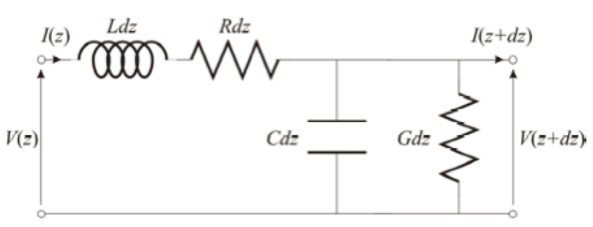
\includegraphics[width=0.5\textwidth]{Images/figure5.png}
\end{center}
Che possiamo sintetizzare in queste equazioni:
\begin{equation*}
    \begin{cases}
    Z_{RL} dZ = R dz + j \w L dz\\
    Y_{GC} dZ = G dz + j \w C dz
    \end{cases}
\end{equation*}
Analizzando la \textbf{maglia} otteniamo:
\begin{equation*}
    V(z) = Z_{RL} dZ I(z) + V(z + dZ)\\
\end{equation*}
Che riscriviamo in questo modo per far uscire un \textbf{rapporto} \textbf{incrementale}:
\begin{equation*}
\begin{aligned}
    V(z + dZ) - &V(z) = - Z_{RL} dz I(z)
    \\
    &\Downarrow \\
    \frac{dV}{dz} = &- Z_{RL} I(Z)
\end{aligned} 
\end{equation*}

Mentre analizzando il \textbf{nodo} otteniamo:
\begin{equation*}
\begin{aligned}
    I(z + dZ) - &I(z) = - Y_{GC} dz V(z)
     \\
    &\Downarrow \\
    \frac{dI}{dz} = &- Y_{GC} V(Z)
\end{aligned}
\end{equation*}
Per rendere queste equazioni simili al caso \textbf{Senza} \textbf{Perdite} si pone:
\begin{itemize}
    \item $L_{EQ} = L - j \frac{R}{\w}$
    \item $C_{EQ} = C - j \frac{G}{\w}$
\end{itemize}
Con cui otteniamo:
\begin{squared}
\tag{Equazioni delle Linee}
\begin{dcases}
    \frac{dV (z)}{dz} = -j \w L_{EQ} I (z) \\
    \frac{dI (z)}{dz} = -j \w C_{EQ} V (z)
\end{dcases}
\end{squared}
Queste equazioni sono analoghe a quelle che legano campo elettrico e magnetico per un'\textbf{Onda} \textbf{Piana} che si propaga nella direzione z, quindi hanno delle \textbf{soluzioni} \textbf{analoghe}:
\begin{equation*}
    I = \frac{1}{-j \w L} \ \frac{dV(z)}{dz} 
\end{equation*}
Che se sostituiamo nella\textbf{ seconda equazione delle Linee} ci restituisce:
\begin{squared}[green]
    \tag{Equazione di Helmotz}
    \frac{d^2V (z)}{dz^2} = -\w^2 LC V 
\end{squared}
Che è un'\textbf{equazione} \textbf{Differenziale} del \textbf{Secondo} \textbf{ordine} e che quindi ha per soluzione:
\begin{equation*}
    \begin{dcases}
    V^+ e^{-jkz}\\
    V^- e^{jkz}
    \end{dcases}
    , \ con \ k = \w \sqrt{LC}
\end{equation*}
\begin{center}
\begin{equation*}
    V(z) = V^+ e^{-jkz} + V^- e^{jkz}
\end{equation*}
\end{center}
Con $V^+ = |V^+|e^{j\varphi^+}$ e $V^- = |V^-|e^{j\varphi^-}$ \textbf{Complesse}\\ \\
Nel \textbf{dominio del Tempo} le due soluzioni diventano:
\begin{equation*}
\begin{aligned}
    v^+(z,t) &= Re\left\{V^+ e^{-jkz} e^{j\w t}\right\} = Re\left\{|V^+|e^{j\varphi^+} e^{-jkz} e^{j\w t}\right\} =\\
    &= |V^+| \cos\left(\w \left(t + \frac{\varphi^+}{\w} \right) - kz \right) =\\
    &=|V^+| \cos\left(\w \left(t - t_0^+ \right) - kz \right) =\\
    &= |V^+| \cos(k(vt - vt_0^+ - z)) 
\end{aligned}
\end{equation*}
Dove:
\begin{itemize}
    \item $t_0^+ = - \frac{\varphi^+}{\w}$
    \item $v = \frac{\w}{k} = \frac{1}{\sqrt{LC}}$
\end{itemize}
\vspace{1cm}
Analogamente per la \textbf{soluzione} \textbf{negativa} faremo:
\begin{equation*}
\begin{aligned}
    v^-(z,t) &= Re\left\{V^- e^{jkz} e^{j\w t}\right\} = Re\left\{|V^-|e^{j\varphi^+} e^{jkz} e^{j\w t}\right\} =\\
    &= |V^-| \cos\left(\w \left(t + \frac{\varphi^-}{\w} \right) + kz \right) =\\
    &=|V^-| \cos\left(\w \left(t - t_0^- \right) + kz \right) =\\
    &= |V^-| \cos(k(vt - vt_0^- + z)) 
\end{aligned}
\end{equation*}
Dove:
\begin{itemize}
    \item $t_0^- = - \frac{\varphi^-}{\w}$
    \item $v = \frac{\w}{k} = \frac{1}{\sqrt{LC}}$
\end{itemize}
Possiamo fare un procedimento del tutto analogo con l'\textbf{equazione di Helmotz della corrente}, per questo capiamo che tensione e corrente sono soluzioni del \textbf{sistema omogeneo di equazioni differenziali}.\\ 

Cominciamo quindi a sostituire la tensione nella prima equazione:
\begin{equation*}
    \frac{dV}{dz} = - j k V^+ e^{-jkz} = -j \w L I
\end{equation*}
\begin{equation*}
    \implies I = \underbrace{\underbrace{\frac{k}{\w L}}_{\frac{1}{Z_0}} V^+}_{I^+} e^{-jkz}
\end{equation*}
Questo vuol dire che se è presente un'\textbf{onda progressiva di tensione} $\left(V^+ e^{-jkz}\right)$ è anche presente un'\textbf{onda progressiva di corrente} $\left(I^+ e^{-jkz}\right)$.\footnote{Un discorso analogo vale per l'onda di tensione che va nel verso opposto.}






